\documentclass[conference]{IEEEtran}
\usepackage[utf8]{inputenc}
\usepackage[T1]{fontenc}
\usepackage{graphicx} % Required for including images
\usepackage{amsmath} % Required for math commands
\usepackage{booktabs} % Required for professional looking tables
\usepackage{float} % Required for tables and figures positioning
\usepackage{xcolor} % Required for color definitions
\usepackage{afterpage}

\definecolor{myblue}{HTML}{717AFD}
\definecolor{myred}{HTML}{F0564A}
\definecolor{mygrey}{HTML}{464546}

\setlength{\parskip}{0.8em} % Adjust space between paragraphs

\newcommand\wordcount{
   \immediate\write18{wordcount.bat \jobname.tex}
   \input{\jobname.wc}
}

\begin{document}

\title{Biosensors Analysis Report: Glucose and Lactate Biosensors}
\author{Blind grading number 2504F}
\maketitle

\section{Part A: Glucose Biosensors}
\subsection{Introduction}
\IEEEPARstart{G}{lucose} biosensors are vital for managing diabetes, currently aiding over 500 
million patients worldwide in making daily health decisions \cite{GlobalDiabetesCases}. Over the years, these devices
 have undergone significant improvements to provide quick and accurate blood sugar measurements outside of 
 medical facilities. Functioning as compact labs, they detect and measure glucose in biological samples
 and convert this data into electrical signals that are simple to read and interpret \cite{couletWhatBiosensor1991}. 
The evolution from large, lab-based tools to today's handy, portable monitors is a testament to major advancements in technology.

Glucose biosensors have come a long way since the first lab-based Yellow Springs Instrument\cite{chuaPlasmaGlucoseMeasurement1978}. Today's models are portable, 
allowing people to check their glucose anytime. This change was largely due to glucose oxidase, an enzyme robust and stable enough to 
work outside the lab, leading to smaller, user-friendly devices for everyday use \cite{clarkElectrodeSystemsContinuous1962}.

Glucose biosensors, integral to diabetic care, are comprised of four main modules: (1) a potentiostat for the conversion of electrical signals, 
(2) a slot for connecting test strips, (3) a calibration component to ensure accurate glucose measurements, and (4) an optional display module for user interaction. 
Embedded within the potentiostat electrode, the enzyme glucose oxidase initiates a reaction with glucose to produce gluconolactone, while an 
artificial mediator undergoes reduction and subsequent reoxidation, generating a current that corresponds to the glucose concentration. 
Numerous advancements have been integrated into glucose oxidase biosensors, with one significant enhancement being the introduction of ferrocene as an 
electron acceptor instead of oxygen, which has rendered the sensing reaction more efficient and less susceptible to interference from oxygen fluctuations 
(Figure \ref{fig:initialdiagram}).

\begin{figure}[h]
   \centering
   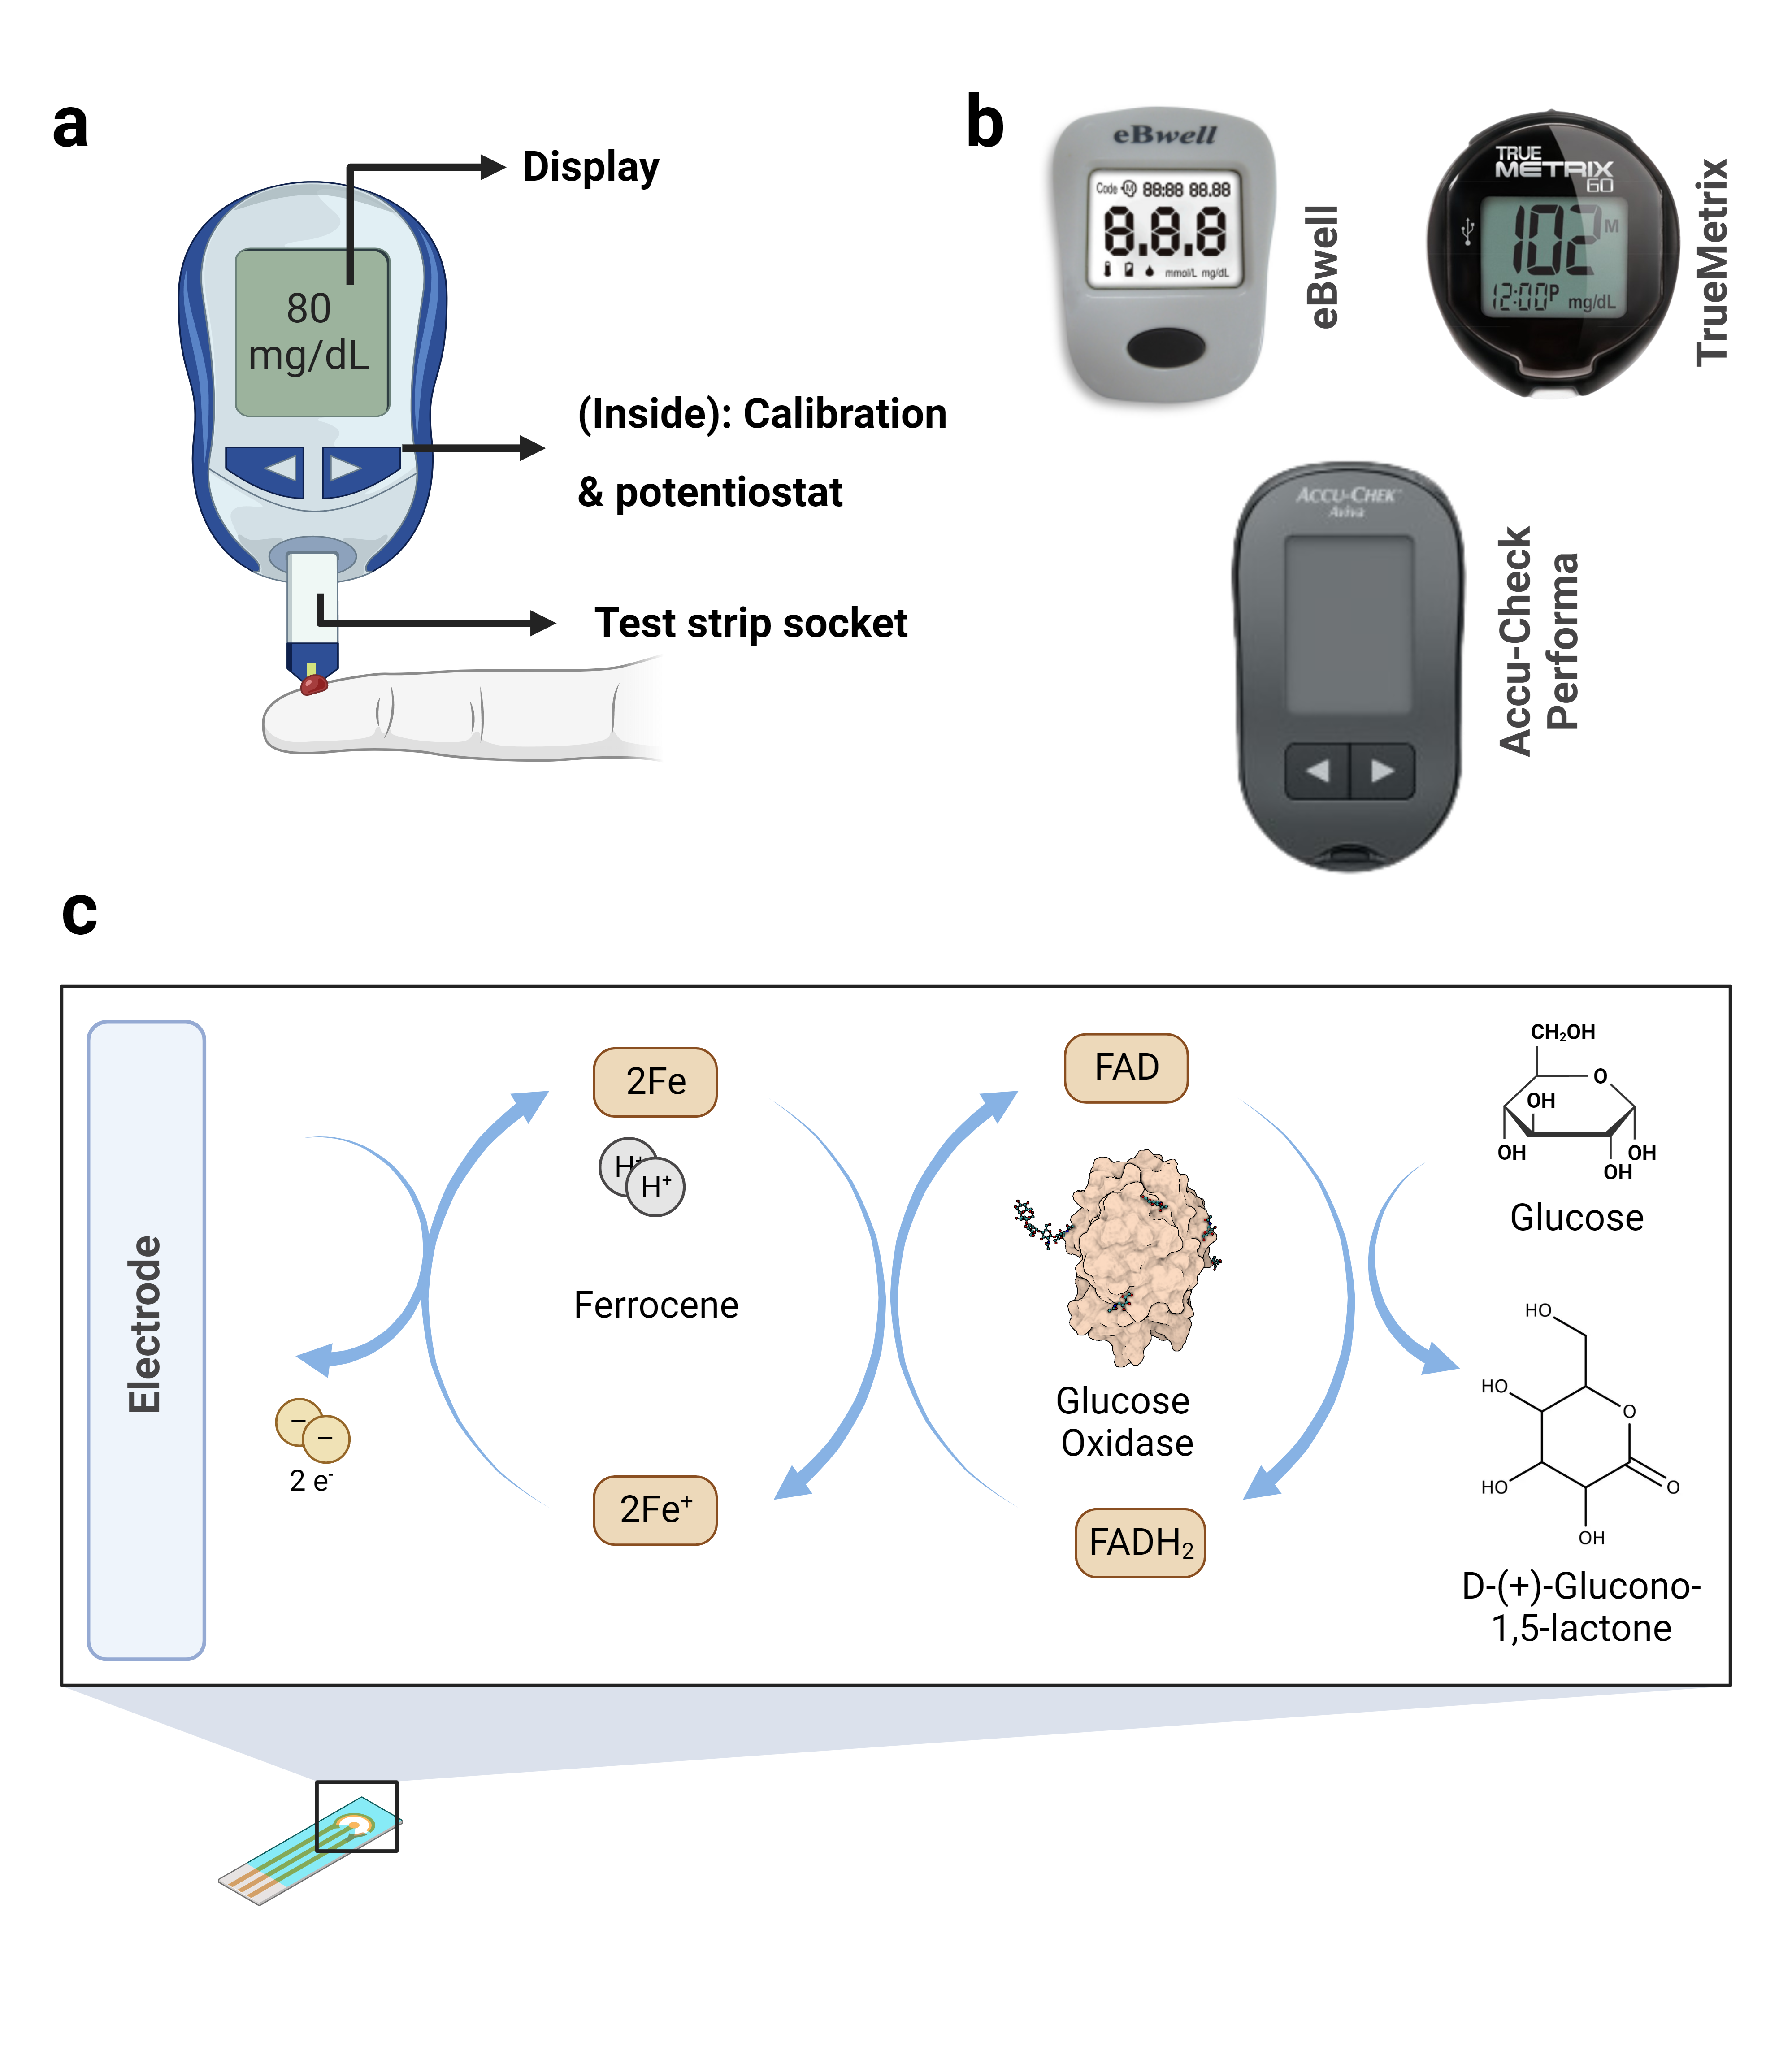
\includegraphics[width=1\linewidth]{images/initial diagram.png}
   \caption{Schematic Overview of a Glucose Biosensor. 
   (a) External view of a typical glucose monitor. (b) Top view of the three commercial biosensors assessed during this report.
   (c) Diagram of the enzymatic reaction pathway inside the biosensor, where glucose oxidase 
    catalyzes the conversion of glucose to gluconolactone, with ferrocene acting as an artificial 
    electron acceptor, to end in an electrical signal at the electrode.}
   \label{fig:initialdiagram}
\end{figure}

In addition to the core technical parameters such as accuracy, precision, and limit of detection (LoD) that define the functionality of 
glucose biosensors, qualitative aspects related to user experience and device handling play a major role in determining the reliability 
of the results. Even with the most advanced technology, the outcome of a measurement will always be compromised by mishandling or improper use. 
Therefore, the User Experience/User Interaction analysis (UX/UI) is one of the most important design principles of these devices, focusing on ease 
of use and intuitive interaction, as accurate readings are not just a matter of sophisticated technology but also of user-friendly operation.

In this report, we will objectively evaluate three sensors with the aim of (1) assessing their quantitative parameters of precision and accuracy 
(which we will try to correlate with the technology used) and (2) evaluating the product as a whole to determine which one is the most suitable 
for everyday use by a diabetes patient.

\begin{figure*}[!th]
   \afterpage{\clearpage}
   \centering
   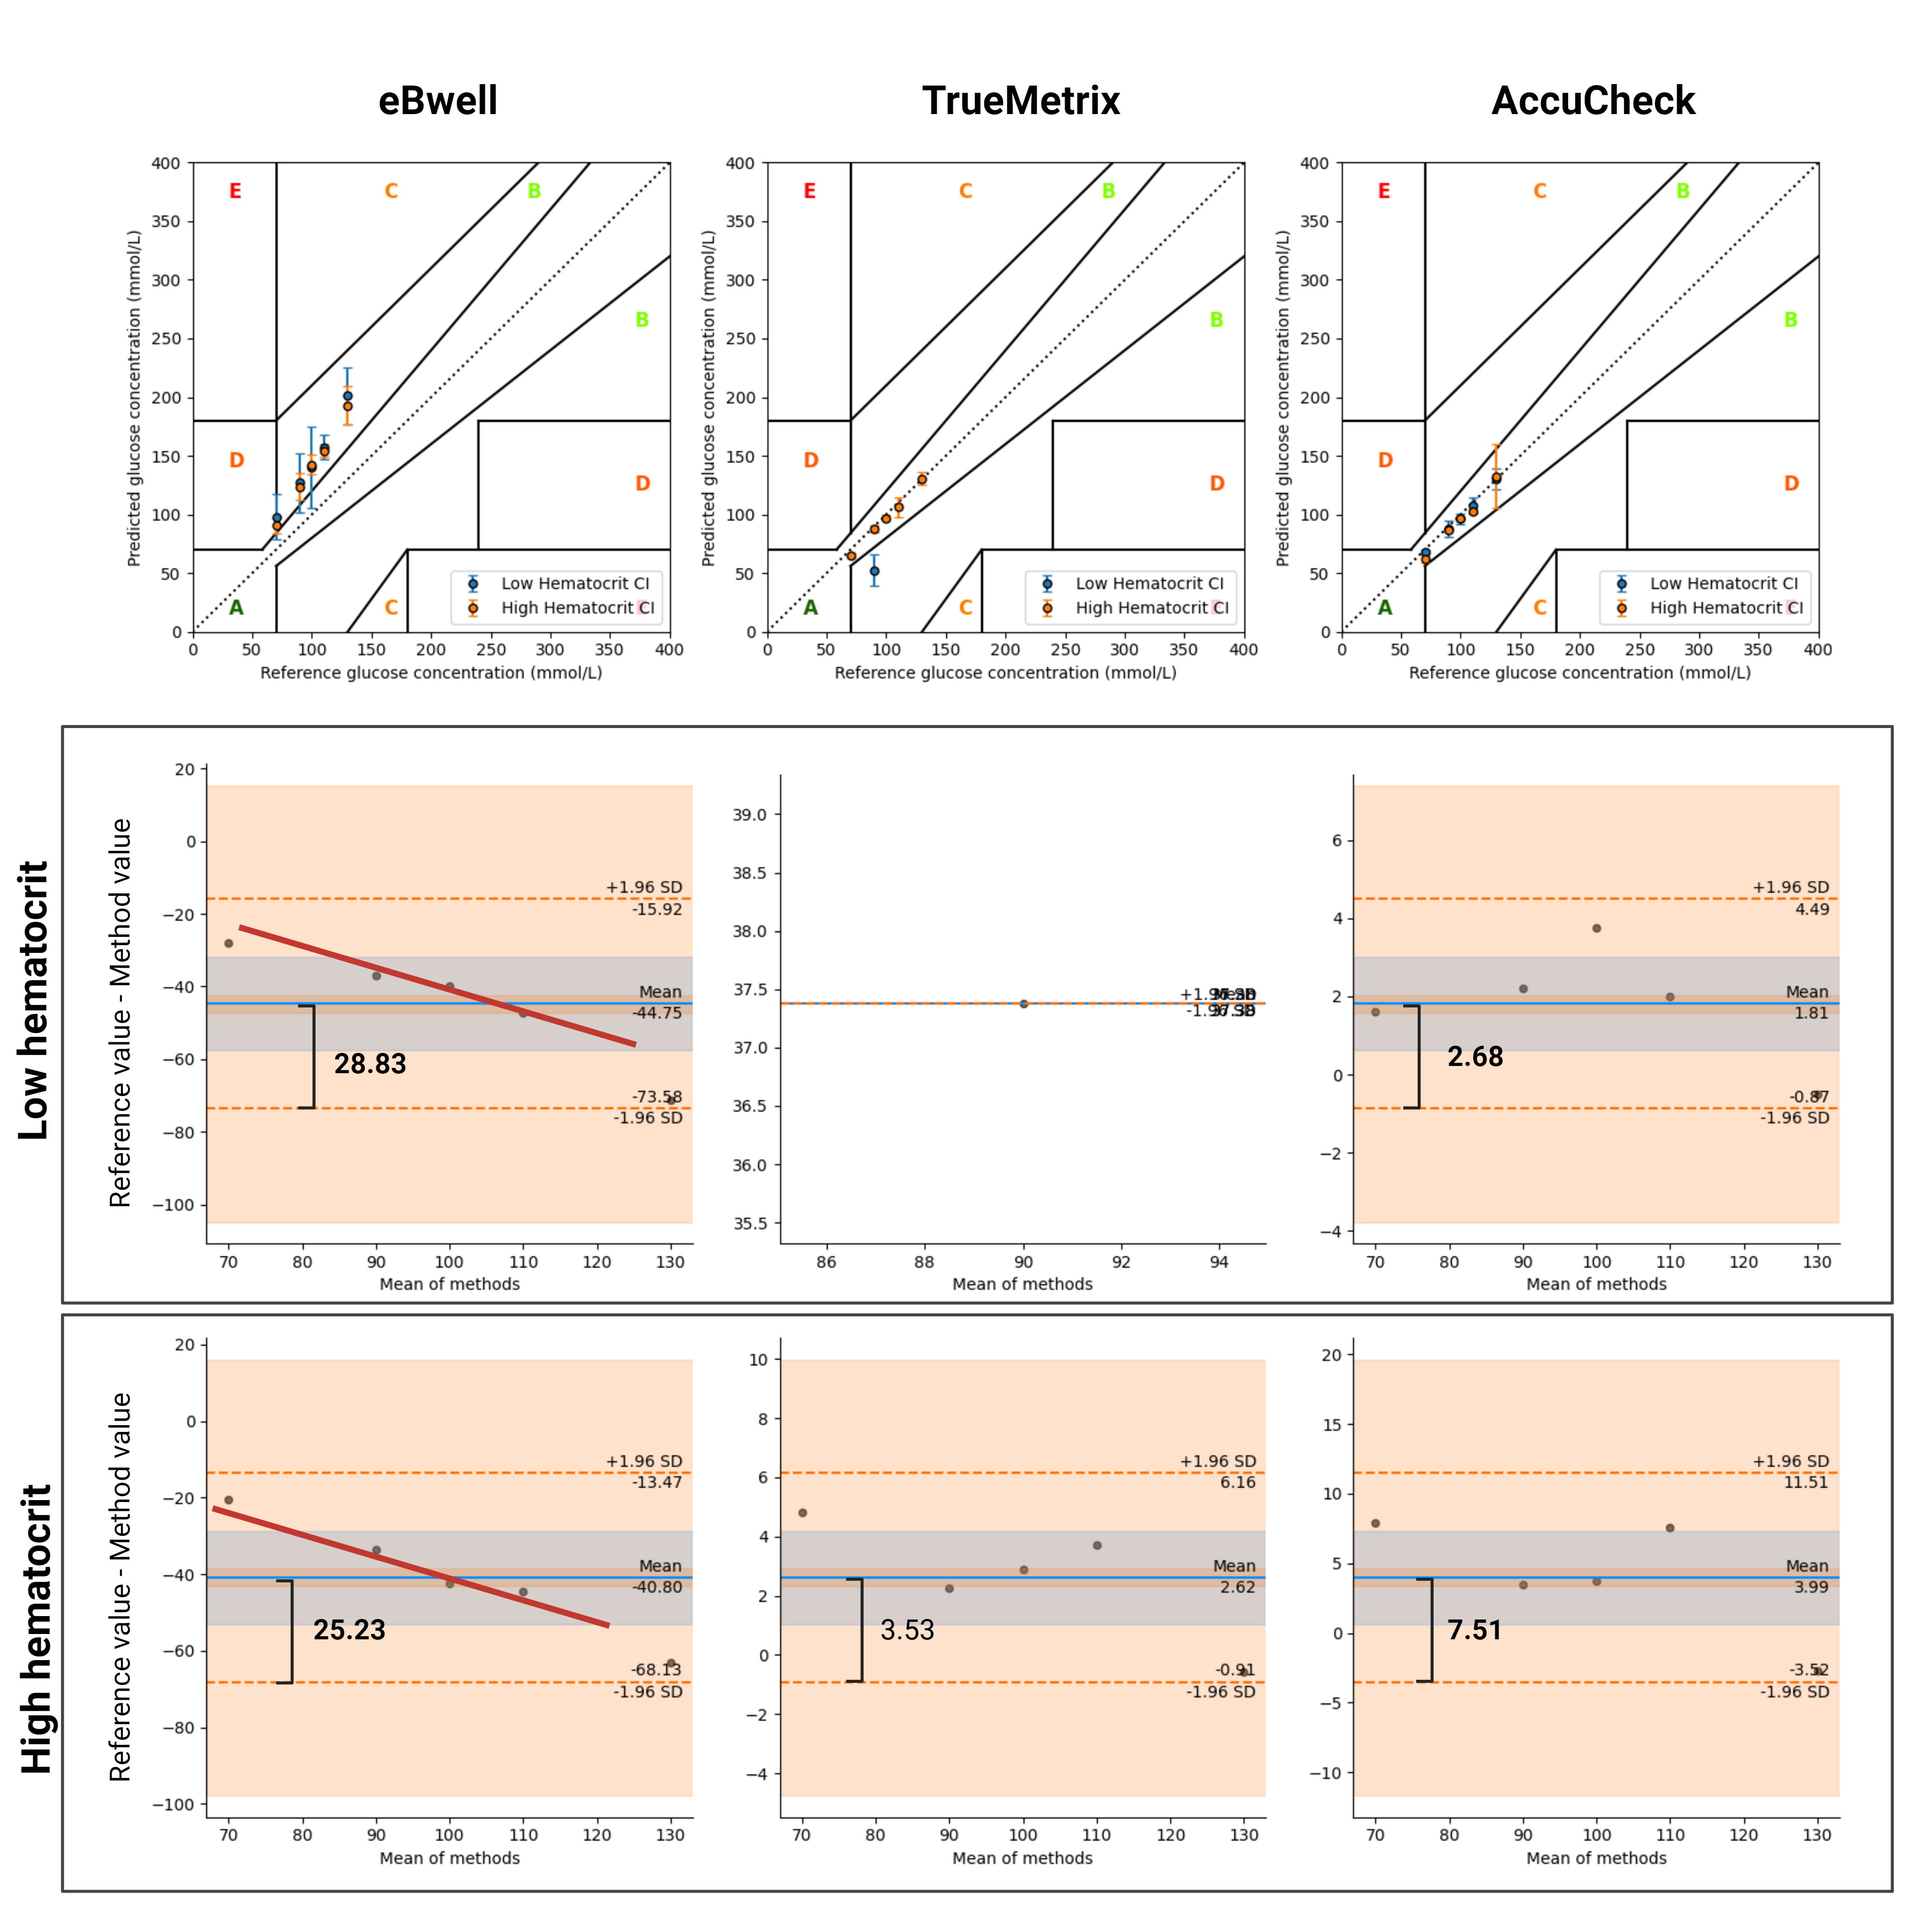
\includegraphics[width=\textwidth]{images/Quantitative results.png}
   \caption{Quantitative analysis of the glucose curve calibration}
   \label{fig:quantitative}
\end{figure*}

\clearpage

\subsection{Materials and Methods}
Glucose meters and test strips were provided, along with samples labeled from A to G, and A* to G* to account for variations in hematocrit levels. 
The strips were utilized for measurement, and the results were critically discussed within the group.

\subsubsection{Concentration of Sugar in Prepared Samples}

\begin{table}[H]
\centering
\caption{Concentration of sugar in prepared samples}
\begin{tabular}{@{}ccc@{}}
\toprule
\textbf{mg/dL Glucose} & \textbf{mM} & \textbf{Sample ID} \\ \midrule
70                     & 3.9         & A, A*              \\
90                     & 5.0         & B, B*              \\
110                    & 6.1         & C, C*              \\
130                    & 7.2         & D, D*              \\
1000 (sucrose)         & 29.2        & F, F*              \\
90 + lemon juice       & 5.0         & G, G*              \\ 
\bottomrule
\\
\multicolumn{3}{l}{\footnotesize *Samples with an asterisk indicate high hematocrit levels.} \\
\multicolumn{3}{l}{\footnotesize *Samples with 'lemon juice' contain relevant traces of citric acid.} \\
\end{tabular}
\label{tab:sugar_concentration}
\end{table}

\subsubsection{Statistical Analysis and Data Visualization}
For the statistical analysis and data visualization, we utilized an open-source Python library \cite{WptmdoornMethcompPython} to generates
 Clarke Error Grid and Bland-Altman plots.

The Clarke Error Grid analysis evidenciate the clinical significance of the differences 
between the measured glucose values and the reference standards. It allowed us to categorize the measurement errors 
and evaluate the potential impact on clinical decision-making.

The Bland-Altman plots offered a graphical method to analyze the agreement between the glucose meters and the reference method.
 By plotting the difference against the average of the two methods, we could assess the precision and identify any systematic bias present in the measurements.   

 \subsection{Results and Analysis}
 % Present and discuss the results from glucose biosensor experiments
 \subsubsection{Quantitative analysis}
 As outlined in the Materials and Methods section, we used Clarke Error Grids and Bland-Altman plots to analyze and display the performance of different methods compared with the reference values. 
 The Clarke Error Grid was utilized to visualize data distribution against the reference value and assess its clinical decision-making impact, while Bland-Altman plots were employed to compare
 error distributions (including means and confidence intervals) and identify error patterns (refer to Figure~\ref{fig:quantitative}).

 Following this analysis, the observed patterns are as follows:
 
 \begin{enumerate}
     \item \textbf{eBwell:} This device exhibited the highest absolute error (lack of accuracy) and a lack of precision, as evidenced by the higher standard variance between 
     replicates. The Bland-Altman plot indicates a negative coefficient of error progression with increasing glucose levels, suggesting a growing overestimation relative to 
     the reference value. At low glucose concentrations, some measurements fall into the clinically dangerous Zone D, posing significant risks in hypoglycemia detection. 
     Despite entering Zone B at high glucose concentrations, which denotes more than a 20\% deviation, the diagnostic outcome remains unchanged. A comparison of Bland-Altman 
     plots for different hematocrit levels and the error bars in the Clarke Error Grids suggests that the sensor's accuracy diminishes with lower hematocrit values.
     
     \item \textbf{TrueMetrix:} The device's primary issue is its inability to measure samples with low hematocrit concentrations, as indicated by the majority of initial data
      points generating an "Error-0" message—interpreted as "Low Hematocrit" according to the manual. For high hematocrit samples, TrueMetrix showed the highest precision and, 
      along with AccuCheck, the best accuracy.
     
     \item \textbf{AccuCheck:} Across the board, AccuCheck demonstrated the most favorable precision and accuracy. The Clarke Error Grids reveal that samples are well-centered
      in comparison to the reference value, with mean and confidence intervals not straying into unsafe grid regions. The sole exception is the highest glucose sample with high
       hematocrit, which, despite more significant replicate dispersion, sees its confidence interval marginally touching Zone B, not indicative of a diagnostic error.
 \end{enumerate}

 \subsubsection{Unexpected results and other relevant data}
 \begin{enumerate}
   \item \textbf{Effect of Lemon Juice:} Sample G* is unique because it initially contains a glucose concentration of 90 mg/dL (equivalent to 5 mM), which is then altered by adding lemon juice though the precise composition is not quantified. 
   After adding lemon juice, AccuCheck either displays Err-3 (indicating the test strip was exposed to air for too long)
   when hematocrit is low, or shows saturated glucose levels (when hematocrit is high), while eBwell consistently indicates high glucose content, saturating its measurements. On the other hand, the case of TrueMetrix is definitely interesting.
   While the device normally cannot measure any low-hematocrit concentration, when lemon juice is added, the device seems to recover some signal, probably generated by an unspecific interaction with the ascorbic acid that enables the device to bypass its hematocrit
   safety controls. The most plausible explanation is that chemical species such as ascorbic acid present in the juice act as an alternative reducing agent, instead of the glucose oxidase/dehydrogenase, donating electrons to the reaction in the absence of glucose.
   \item \textbf{All the sensors are insensitive to sucrose:} While solution F/F* 
   is labeled as having a concentration of '1000mg/dL' and being 'sugary,' 
   every monitor consistently indicates 'ERROR' or 'LOW' results. The key 
   factor influencing these readings is the type of sugar present—a high 
   concentration of sucrose rather than glucose. The glucose 
   oxidase/dehydrogenase within the sensors is specifically designed to 
   react solely with glucose as the target analyte. Since sucrose is a 
   disaccharide composed of fructose and glucose, without hydrolyzing the 
   bond between them, it cannot be catalyzed by the enzyme. Consequently, 
   the 'LOW' reading displayed by the monitors is entirely justified, given 
   that the glucose concentration in solution F/F* is effectively zero.   
     \item \textbf{High Err-2 Occurrence in TrueMetrix:} In our experience error-2 is mostly caused by a significant difference in the usage mode of TrueMetrix compared to other sensors. This device requires the user to 
     immerse the strip and keep it submerged until the screen displays three lines. Despite being mentioned in the user manual once, the high number of errors suggests that it is not intuitive, and if the 
     user reads the manual briefly, there is a high probability of using the device incorrectly. 
   \end{enumerate}

 \subsubsection{Qualitative analysis}

 To conclude our practices, our team considered not only the precision and 
 accuracy of the biosensors but also their qualitative attributes. After a 
 thorough evaluation of the three sensors, it became evident the importance of non-quantitative 
 characteristics that contribute to the overall user experience and their impact 
 on outcomes. As previously mentioned, improper use of a device can lead to 
 significantly greater errors (and therefore increased risk) than a device with 
 minor precision errors but is much more intuitive to use.
 
 In terms of ease of use, Accu-Chek emerged as the preferred device due to its 
 intuitive design and clear instructions, making it user-friendly. In contrast, 
 TrueMetrix fell short in user acceptance and ease of use. Each group found 
 numerous errors due to misunderstandings about how to handle this initially 
 counterintuitive device, which differs from the other two in the way to 
 present the device to the samples. While the difference is subtle, is key 
 to adquire relevant results and we felt that the instructions did not adequately emphasize these differences in usage. 
 Furthermore, when multiple "err-2" errors appeared due to this issue, there was no 
 indication on the error page that point a potential improper handling cause, but rather an standard origin.
 
 
    \begin{figure}[htbp]
      \centering
      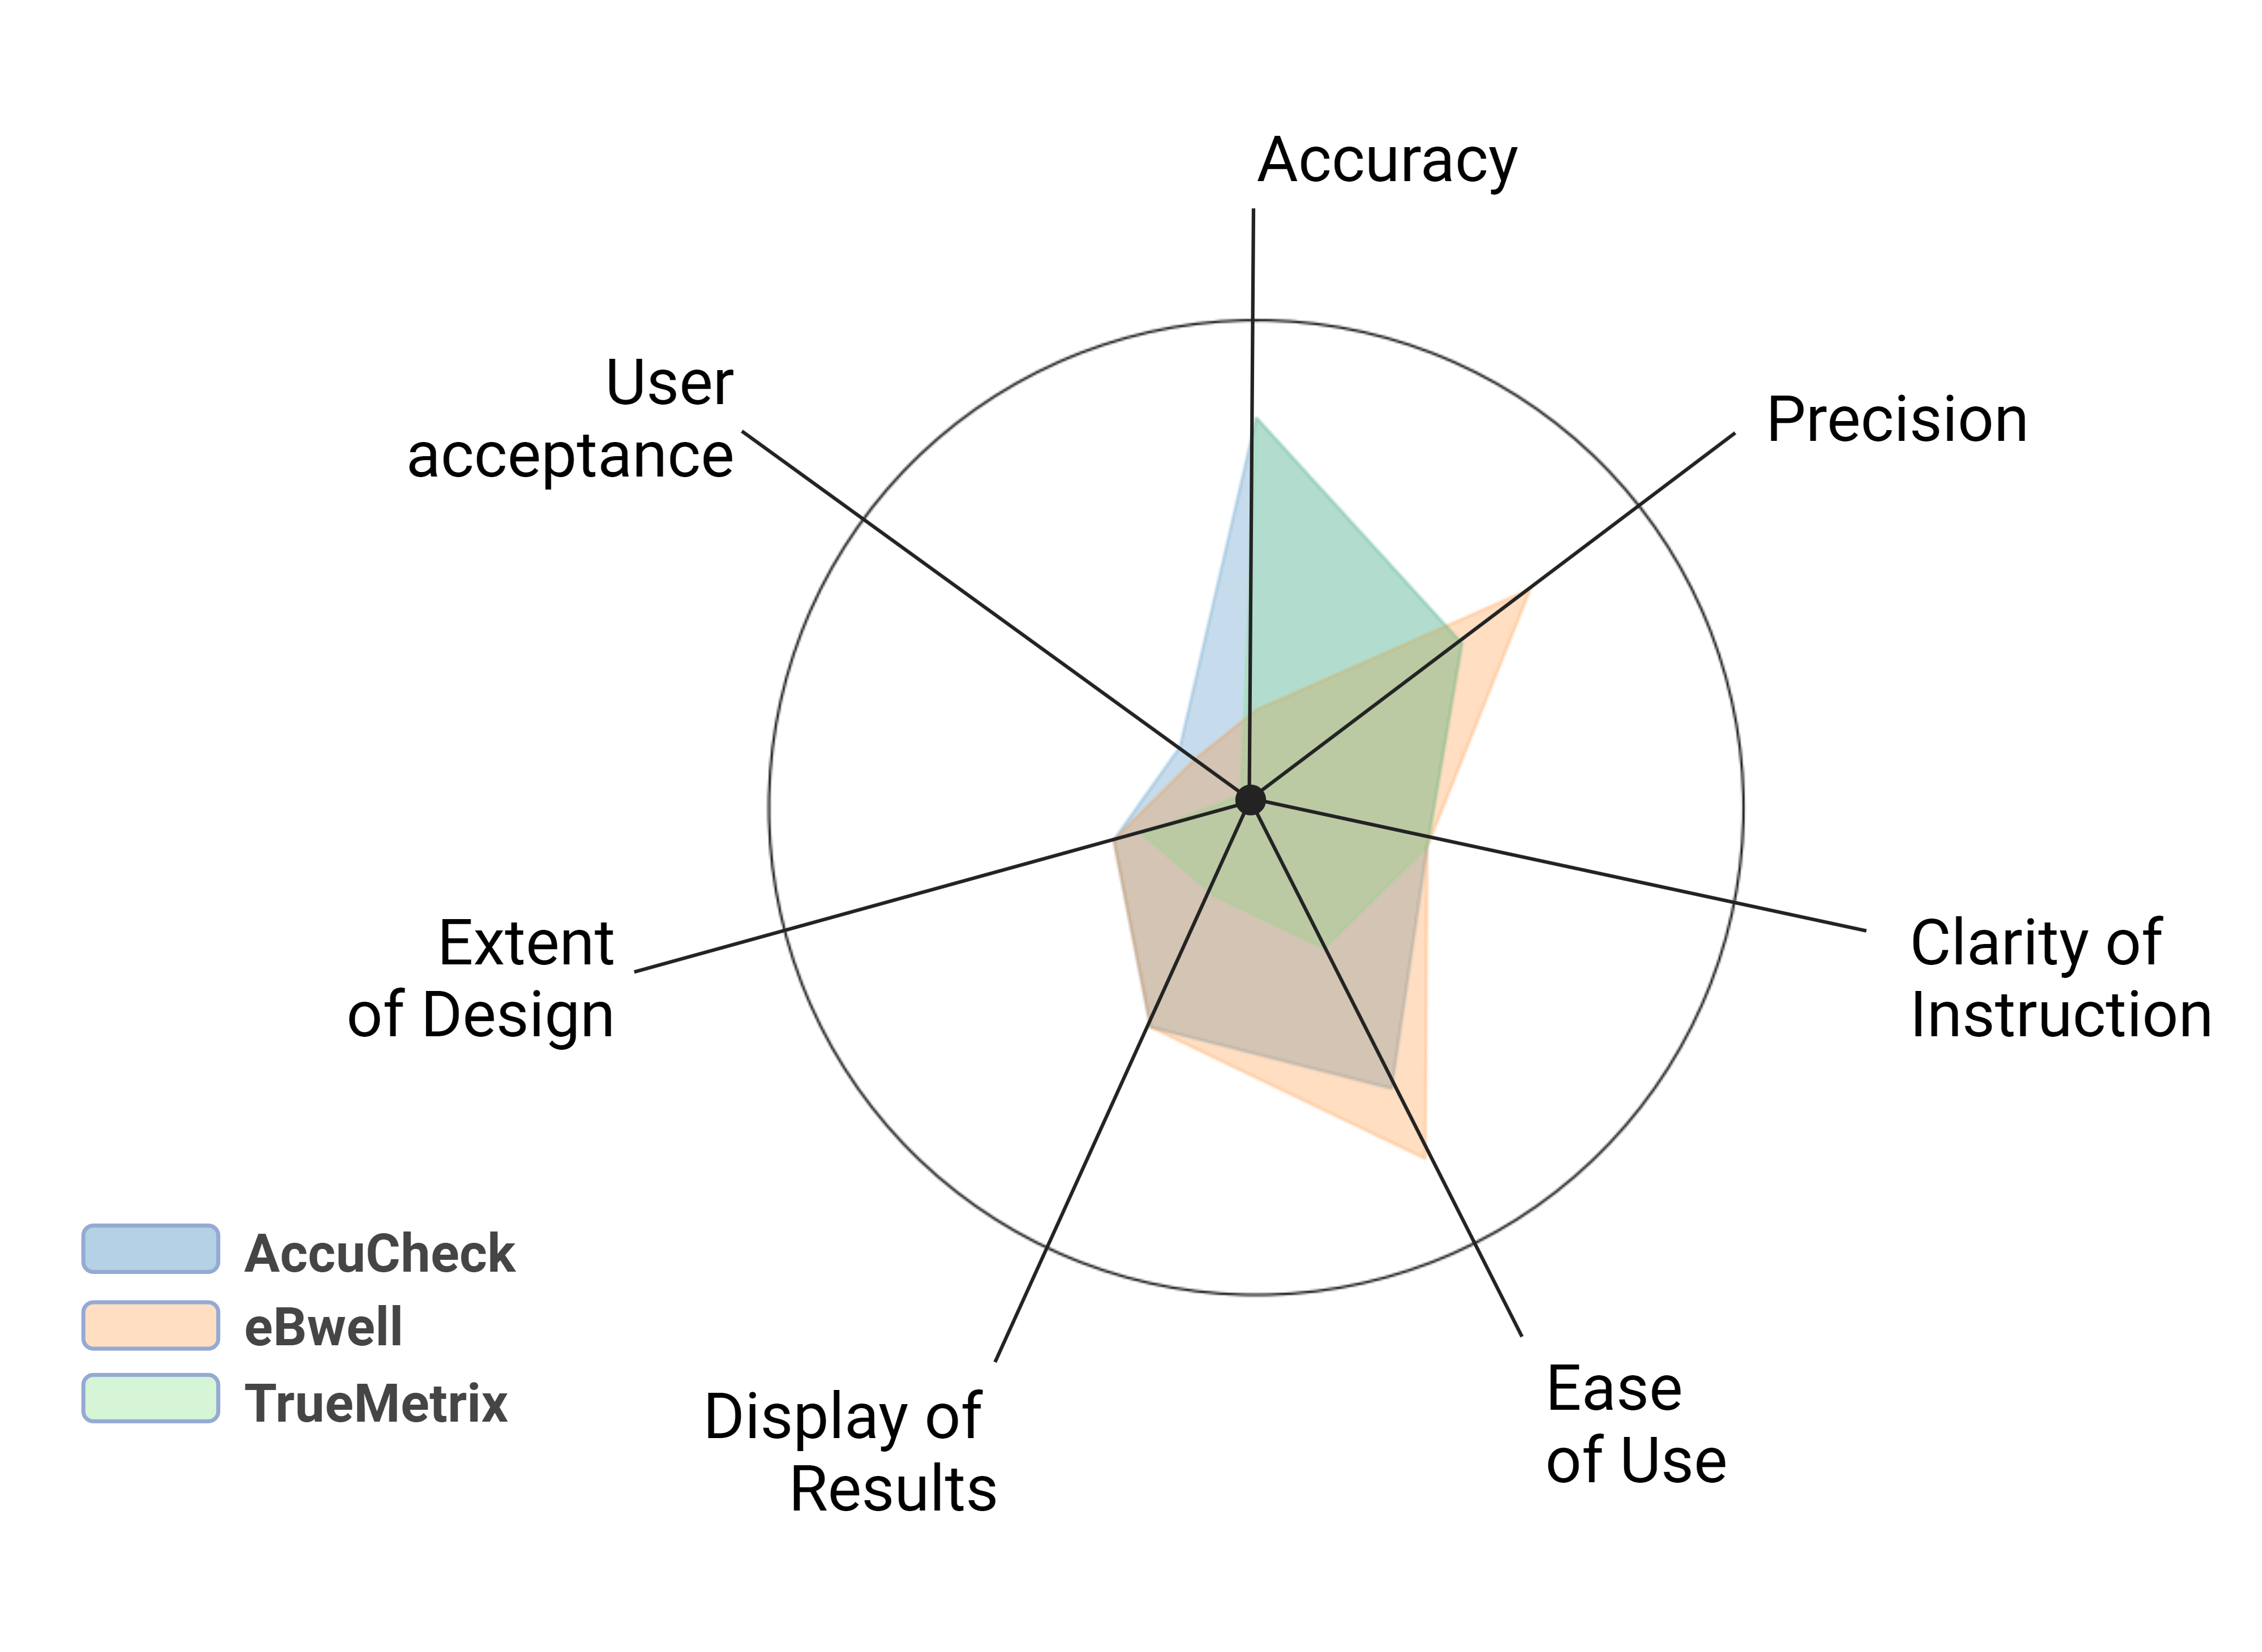
\includegraphics[width=0.9\columnwidth]{images/qualitative.png}
      \caption{Visual radar plot of the qualitative analysis of the results.}
      \label{fig:qualitative}
   \end{figure}

   \begin{table}[h]
      \centering
      \caption{Weighted Scores of Glucose Monitors}
      \label{tab:weighted_scores}
      \begin{tabular}{lccc}
      \hline
      \textbf{Parameter} & \textbf{Accu-Check} & \textbf{eBWell} & \textbf{True Metrix} \\
      \hline
      Accuracy & 40 & 10 & 40 \\
      Precision & 27 & 36 & 9 \\
      Clarity of Instruction & 18 & 18 & 18 \\
      Ease of Use & 32 & 40 & 16 \\
      Display of Result & 25 & 25 & 10 \\
      Extent of Design & 15 & 15 & 12 \\
      User Acceptance & 10 & 8 & 2 \\
      \hline
      \textbf{Weighted Total} & 167 & 152 & 119 \\
      \hline
      \end{tabular}
      \end{table}

      The initial evaluation and scoring of the biosensors, conducted after the class and before detailed analysis, 
      might have missed key aspects, especially regarding TrueMetrix and eBWell. The scoring for TrueMetrix's precision 
      and accuracy needs reevaluation due to its poor performance with low hematocrit values, often leading to missed measurements. 
      eBWell's precision score also requires revision owing to its consistent bias that grows with increasing glucose levels. 
      In summary, the accuracy and precision ratings of both devices need adjustments to more accurately reflect their performance, 
      as opposed to AccuCheck, which demonstrated satisfactory results.
   
 
 \subsection{Discussions}
 In summary, our comprehensive analysis of glucose biosensors has highlighted 
 the critical balance between technical performance and user-centric design. 
 While the quantitative aspects such as accuracy, precision, and detection 
 limits are fundamental in ensuring reliable measurements, the qualitative 
 aspects, particularly ease of use and clarity of instructions, play an equally 
 vital role in ensuring the effective application of these devices in real-world 
 scenarios. The case of TrueMetrix illustrates how design and user interface 
 shortcomings can lead to a high incidence of user errors, undermining its 
 overall efficacy. Conversely, Accu-Chek's superior performance across both 
 quantitative and qualitative parameters underscores the significance of an 
 intuitive design and clear instructions, which enhance user experience and 
 thereby the reliability of the readings. This emphasizes the necessity for 
 manufacturers to invest not only in technological advancements but also in 
 user-friendly design to ensure the broader acceptance and effective utilization 
 of their products.
 
 Furthermore, the unexpected results observed, such as the impact of external 
 factors like lemon juice on glucose readings (been able to even bypass the low hematocrit error triggers)
  and the insensitivity of the 
 sensors to non-glucose sugars, underscore the importance of comprehensive 
 testing under varied conditions to understand the limitations and potential 
 interferences in real-world applications. The influence of hematocrit levels on 
 glucose measurements, as highlighted in recent research, further illustrates 
 the complex nature of these devices and the need for meticulous design and 
 testing. These findings suggest a need for ongoing research and development to 
 refine biosensor technology, addressing not only the fundamental sensing 
 mechanisms but also factors influencing user interaction and external 
 environmental impacts. As biosensors continue to evolve, a holistic approach 
 that encompasses both the technical and human aspects of device usage will be 
 crucial in developing reliable, user-friendly devices that can be seamlessly 
 integrated into personal health monitoring, thereby improving the quality of 
 life for individuals with conditions like diabetes.
 
\section{Part B: Lactate Biosensors}

\subsection{Introduction}

In this section It will be described some ideas to adapt the design principles of 
the AccuCheck glucose sensor, proven in the previous section to have 
superior performance compared to the others, to develop an efficient 
and reliable biosensor for lactate measurement.

The task particularly involves exploring the potential market for lactic acid 
measurement in different biological fluids: blood, cerebral spinal fluid 
(CSF), and sweat. There are two primary markets of interest:

a) The athletic performance market, where lactate levels are indicative of 
the status of anaerobic metabolism during muscle stimulation. This 
information is crucial for athletes aiming to optimize their training and 
performance.

b) The medical diagnostics market, particularly for patients in shock or at 
risk of sepsis and other serious conditions such as meningitis. In these 
scenarios, monitoring lactate levels is vital for timely and accurate 
diagnosis and treatment.

In this regard, the use of cerebral spinal fluid is initially discarded, as the 
very difficulty in its extraction would greatly limit the development of a 
Point of Care product that could be used easily, following the target of 
the AccuCheck sensor.

However, for the other two types of samples, blood and sweat, the sensor 
is already perfectly adapted. Building on this, the main design principle would be to 
create a versatile and accessible lactate biosensor that could reuse as much technological background as possible 
from the AccuCheck glucose sensor.

\subsection{Enzyme election}
During the enzyme selection the main design principles have been maximizing robustness, minimizing complexity and
reusing as many of the existing components in the sensor as possible.Following this idea I've chosen L lactate dehydrogenase (l-LDH, E1.1.1.27) instead 
of lactate oxidase (LOD) because it offers several specific operational advantages; as LOD produces hydrogen 
peroxide as a by-product, which requires a high oxidation potential it makes the system 
susceptible to interference from substances that can be oxidized electrochemically but also makes the system rely in having stable oxigen levels
 \cite{ratheeBiosensorsBasedElectrochemical2015}. 

In contrast, l-LDH uses a coenzyme (NAD or NADP) to facilitate electron transfer between the enzyme and 
the final electron mediator, providing a more stable and interference-resistant pathway. This enzyme converts l-lactate 
to pyruvate while simultaneously reducing NAD to NADH. When NADH reaches the mediator, this one it's oxidized later on on the electrode surface
at a controlled potential, and the resulting current directly and proportionally indicates the l-lactate 
concentration (Figure \ref{fig:reaction}). 

When it comes to the election of D-LDH or L-LDH, I have chosen to focus on L-lactate sensing because it is the predominant form produced in human metabolism,
 making it the primary target for measurement. Elevated levels of L-lactate often indicate an increased reliance on anaerobic
  metabolism due to tissue hypoperfusion. In contrast, D-lactate, which is produced as a byproduct of bacterial metabolism, 
  is more relevant in too specific clinical scenarios, such as patients with short-gut syndrome or a history of gastric 
  bypass or small-bowel resection. \cite{LacticAcidosisBackground2020}.

\begin{figure}[t]
   \centering
   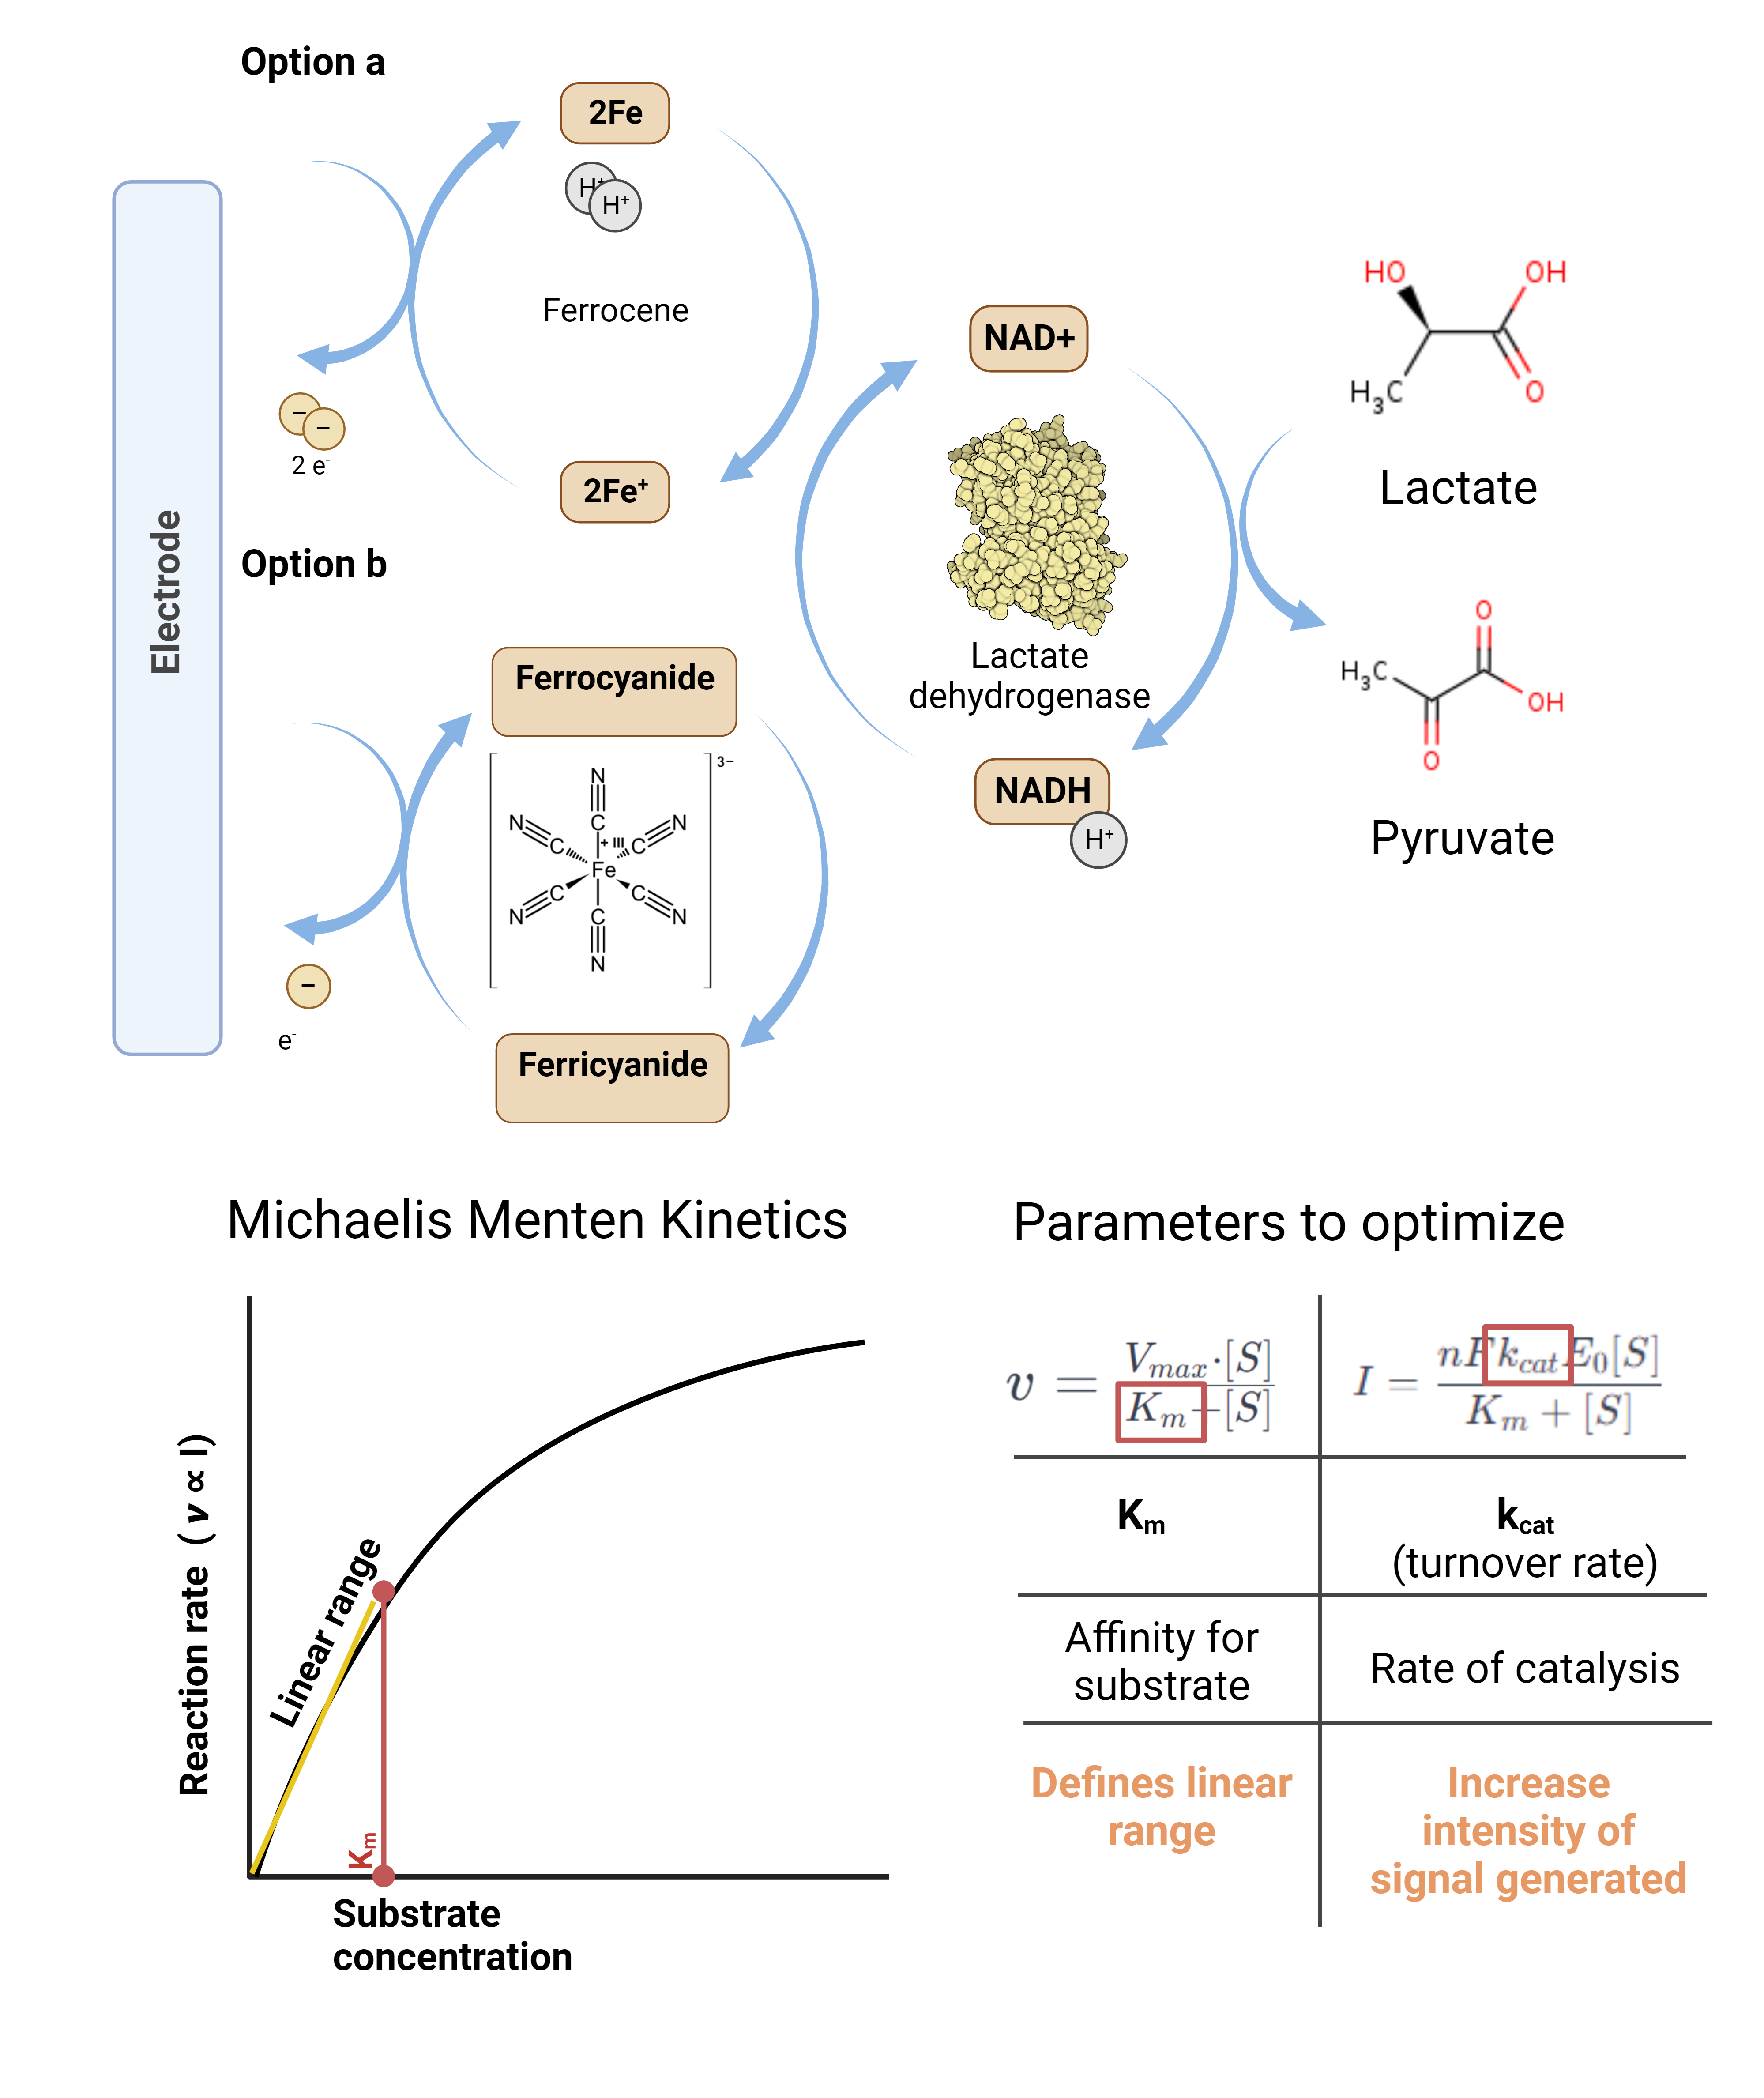
\includegraphics[width=0.9\columnwidth]{images/reaction.png}
   \caption{(Top) Comparative Schematic of Electron Transfer Mechanisms and Enzyme Kinetics in Bioelectrocatalysis:
   Evaluating the pathways of electron shuttling via ferrocene and ferrocyanide (Options a and b) in conjunction 
   with lactate dehydrogenase-mediated conversion of lactate to pyruvate. (Bottom) Illustrating the Michaelis-Menten 
   kinetics with parameters for optimizing the reaction efficiency and enzyme election.}
   \label{fig:reaction}
\end{figure}

To specifically choose the source organism of the enzyme and its subvariant, initially I decided optimize two parameters: the affinity constant (\(K_m\))
 and the catalysis constant (\(k_{\text{cat}}\)), and later on I included physiological working ranges (as temperature or pH) to match the human ones.

The \(K_m\) defines the affinity with which the enzyme binds to the substrate, upon which it depens the linear response range of the reaction. 
Therefore, the choice of this \(K_m\) should be informed by the physiological ranges of lactate in different tissues:

- When measuring \textbf{performance in athletes}, it is important to detect when pyruvate starts to accumulate, in order to prevent its overproduction before 
it crosses the threshold point, where the rate of lactate generation is higher than its clearance rate. This is why, even though the physiological 
ranges of lactate in sweat oscillate between 1-25 mM \cite{derbyshireLactateHumanSweat2012}, the sensor must be capable of quantifying the smallest 
possible change to detect the lactate growth as early as possible.

- When measuring lactate for \textbf{medical purposes}, the sensor needs to operate at the upper limit of normal blood lactate levels, to detect when they reach
 or begin to exceed these levels. Normal levels reach up to 2 mM \cite{LacticAcidosisBackground2020}, levels higher than this are indicative of various
  diseases, with the most severe cases capable of raising lactate levels to 4 mM.

In this regard, \(K_m\) marks the upper limit of the linear region, so I first filtered enzymes with \(K_m\) values right in the upper limits of the regions where we want
 to be linear. A selection of these enzymes and their various parameters and ranges can be found in Table \ref{tab:enzymes_athletic} .

 \begin{table}[h]
   \centering
   \caption{\textbf{Enzyme candidates sorted by \(K_m\)}\cite{InformationEC27}.}
   \label{tab:enzymes_athletic}
   \begin{tabular}{lll}
   \hline
   \textbf{KM [mM]} & \textbf{ORGANISM} & \textbf{COMMENTARY} \\
   \hline
   \multicolumn{3}{l}{Athletic performance candidates (low \(K_m\))} \\
   \hline
   0.0026 & Sus scrofa & pH 8.5, 25°C, isozyme H4 \\
   0.0057 & Sus scrofa & pH 8.5, 25°C, isozyme H2M2 \\
   0.0142 & Sus scrofa & pH 8.5, 25°C, isozyme M4 \\
   0.515 & Epidalea calamita & 15°C, pH 8 \\
   0.517 & Pelophylax perezi & 20°C, pH 8 \\
   \textbf{0.537} & \textbf{Pelophylax perezi} & \textbf{20°C, pH 7.4} \\
   0.541 & Epidalea calamita & 15°C, pH 8 \\
   0.567 & Epidalea calamita & 15°C, pH 7.4 \\
   \hline
   \multicolumn{3}{l}{\textbf{Medical application candidates (\(K_m\) aprox. 4mM)}} \\
   \hline
   2.5  & Molinema dessetae & - \\
   \textbf{8.1}  & \textbf{Agama stellio stellio} & \textbf{pH 7.5, 25°C} \\
   10.2 & Plasmodium vivax & pH 9.2, 25°C \\
   \hline
   \end{tabular}
   \end{table}
   
   Following these requirements, I have selected the following enzymes:
   \begin{itemize}
      \item For the measurement of athletic performance, as lactate should be detected as soon as possible, before it starts to build up,
       I have opted for the enzyme from \textit{Pelophylax perezi}, with a \(K_m\) of 0.537mM 
      \cite{mendiolaEffectsTemperaturePH1991}. Although this enzyme does not 
      have the lowest \(K_m\), it's the lowest one working at human 
      physiological pH ranges (~7.5). This quite low \(K_m\) presents also a challenge, it might lead to saturation with early concentrations. A potential 
      solution could be to create a mixture of two enzymes on the electrode. 
      One, like \textit{Pelophylax perezi}, would add significant sensitivity, while 
      another one with a higher \(K_m\) will extend the linear range to higher concentrations. When lactate 
      concentration is low, the first enzyme would still detect it effectively, 
      and once the concentration exceeds the linear range of the first enzyme, 
      the second enzyme, less sensitive but with a wider range, would become 
      the principal contributor to generating a linear output.
      
     
     \item For the measurement of lactate in clinical settings, I have chosen the 
     enzyme from the species \textit{Agama stellio stellio}, as it is the enzyme with a 
     \(K_m\) closest to the target range (8.1mM \cite{al-jassabiPurificationKineticProperties2002}) whose optimal pH point is also within 
     the physiological range.
   \end{itemize}

   Unfortunately none of the original publications describe the \(k_{\text{cat}}\) so it remains a parameter to study experimentally.

   Additionally, we would need to choose an expression vector/organism to make a recombinant
production of the protein, as the two model organisms are either an amphibian (\textit{Pelophylax perezi})
or a reptile (\textit{Agama stellio stellio}), and it would be difficult to scale the protein
production relying just on the original host. As both are eukaryotic, a potential organism
would be \textit{P. pastoris}, a yeast widely used for eukaryotic protein production.



\subsection{Mediator}

% ferricyanide? (put paper recommendations) No! ferrocene to rehuse the same than in the strip

Two optional routes are proposed for the mediator (Figure \ref{fig:reaction}), both using NADH as the enzyme's cofactor, but one based on ferrocene and the other on ferricyanide.

The main advantage of using ferrocene is the ability to reuse the same mediator from the previous device. The primary advantage of using ferricyanide is that 
it has a slightly lower Redox potential (0.36V vs 0.4V \cite{cheahElectrochemicalOxidationFerricyanide2021}), which could help lower the potential and prevent 
signal interference from the oxidation of other species. Ferricyanide has been described in previous studies as working in harmony with the same enzyme \cite{nikolausAmperometricLactateBiosensors2008}.


\subsection{Enzyme binding and calibration}

% gold activated with TGA
For enzyme immobilization, as AccuCheck electrodes are based on gold\cite{TestStripFaq}, we could potentially use an approach based on bioactivating 
the electrode surface with a monolayer of thioglycolic acid (TGA), which then will act as a matrix for enzyme immobilization.

Another important variable to optimize is the dimensions of the capillary, which determine 
the diffusion coefficients and potentially extend or narrow the linear range of the electrode (complementing the choice of \(K_m\) of the enzyme). 

Therefore, once the reaction is designed and the enzyme is chosen, a subsequent optimization step would involve the analysis of the sensor's 
linear range while attempting to optimize it by tuning the capillary height.


\begin{figure}[t]
   \centering
   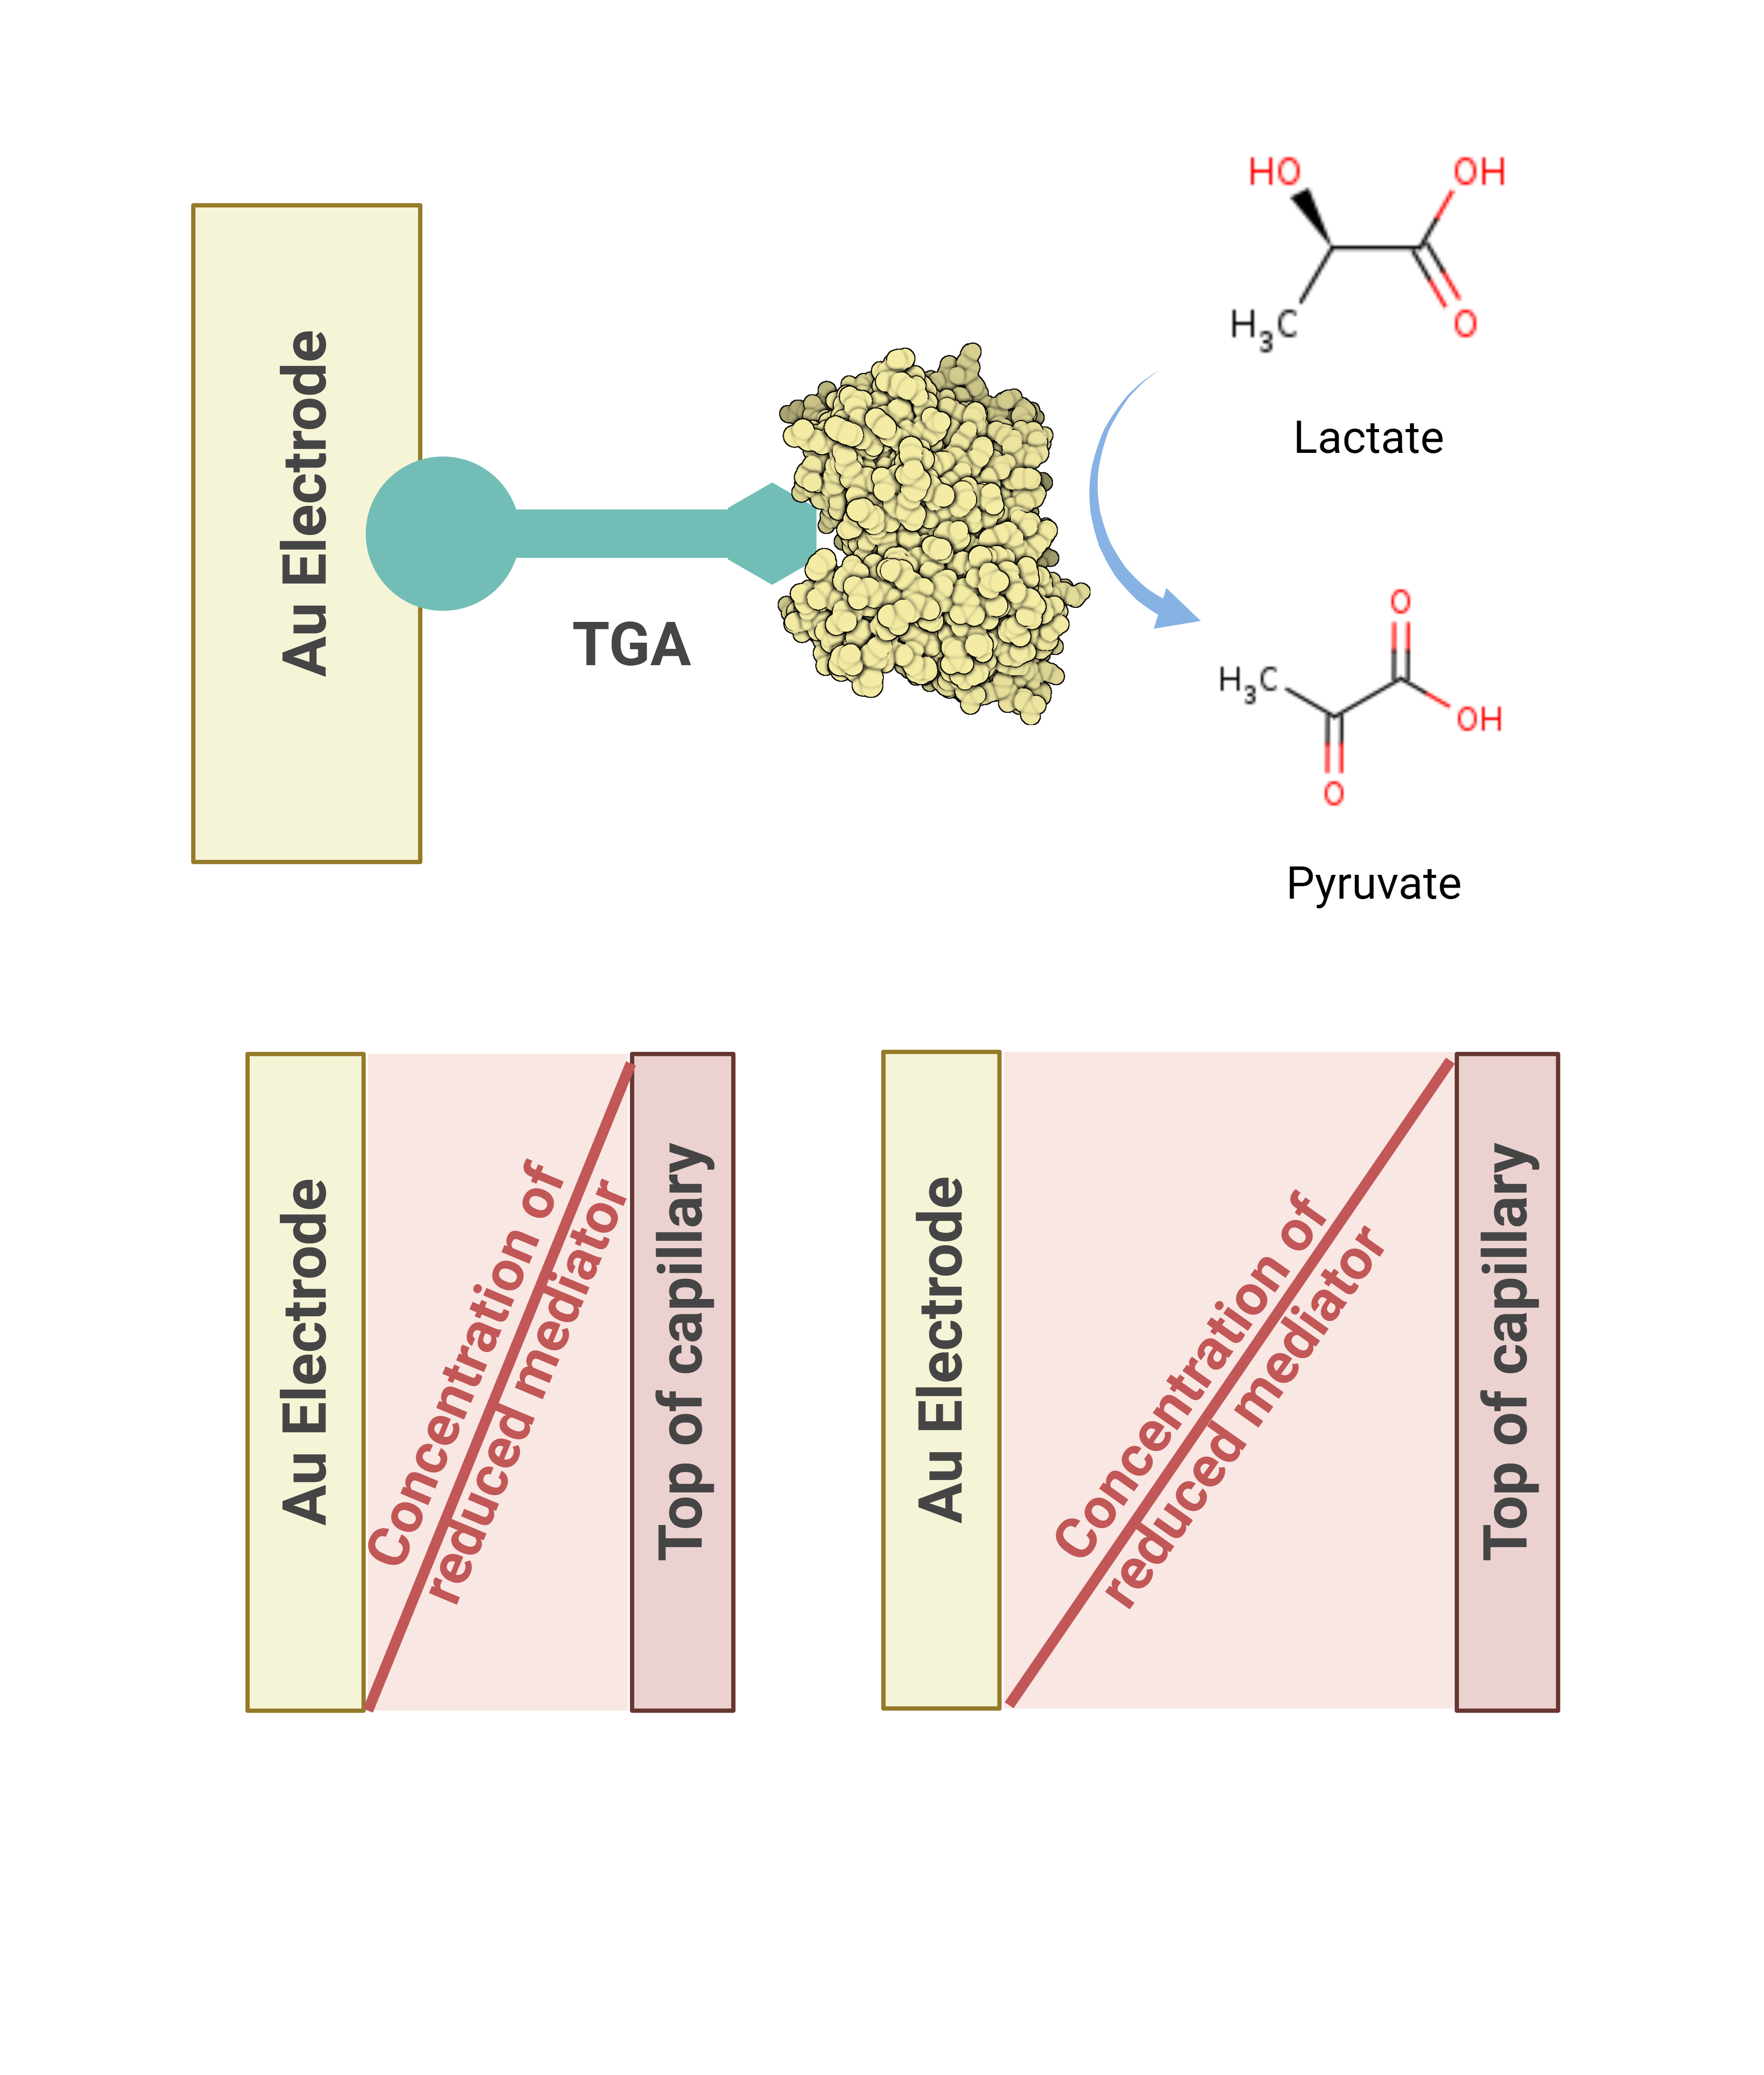
\includegraphics[width=0.9\columnwidth]{images/electrode preparation.png}
   \caption{(Top) Scheme of preotein immobilization over the electrode. (Bottom) Illustration of the effect of the capilary dimension of the diffusion coefficient.}
   \label{fig:reaction}
\end{figure}

Finally, to comply with regulations and understand how safe our sensor is (and in which situations it should be used), we must conduct an analysis similar to the one performed in 
the first part of this report (establishing precision and accuracy analysis). This involves comparing our sensor with a reference method for lactate measurement, such as 
laboratory enzymatic assays (where all the conditions are much more controlled), High-Performance Liquid Chromatography (HPLC), or Gas Chromatography-Mass Spectrometry 
(GC-MS) \cite{toffalettiBloodLactateBiochemistry1991}.

To do this, a calibration curve would be established between the experimental ranges, and the sample would be diluted (blood or sweat) to bring it into known lactate ranges, 
thus generating a representative sample of the real target (with the molecular complexity and cellular components that the real world solution would have). 
Afterward, an analysis similar to the one conducted earlier (for example, using Bland-Altman plots) would be performed to analyze the error distribution of the sensor compared 
to the reference(s) method.


% Thickness of enzyme layer also define calibration. Calibrate experimentally.
% choose reference method, run calibration curves.

\subsection{Conclusions}

In summary, the task of adapting the AccuCheck glucose sensor to measure 
lactate highlights not only the various parameters that 
need tuning but also demonstrates the modularity of many market biosensors. 
Reinventing the wheel isn't always necessary; understanding the sensor's 
different modules, instead of treating them as a black box, allows for their 
use in a modular way. 

Specifically, the careful selection of different enzymes, particularly different forms of L-lactate 
dehydrogenase, for various applications in sports performance and medical 
testing, underscores the importance of context in balancing precision and ranges of detection.
 The use of ferrocene or ferricyanide as a conducting agent 
illustrates how decisions sometimes need to find a sweet spot between optimizing sensitivity 
while reusing proven technology.

Moreover, the meticulous attention to details such as the sizing of capillaries 
and the calibration techniques employed emphasizes how mechanical 
aspects are crucial for fine-tuning the system before its real-world 
application.

All these details highlight the importance of considering every aspect of 
sensor design, from the molecular level to the user interface, to achieve an
 outcome that is suitable for real world scenarios.



\bibliographystyle{IEEEtran}
\bibliography{report2_biosensors}

% Uncomment the compliance section if you have set it up properly
\section{Compliance}
\wordcount
\section{Post-Script}
\begin{figure}[h]
   \centering
   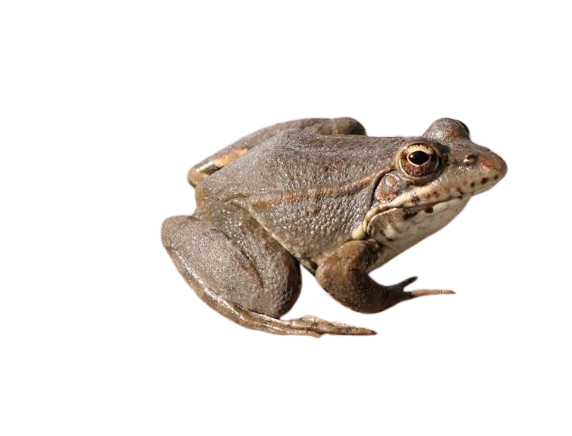
\includegraphics[width=0.9\columnwidth]{images/frog.png}
   \caption{Perez's frog (La rana Pérez; \textit{Pelophylax perezi}), host organism of the employed, super-sensitive, L-LDH enzyme.}
   \label{fig:perezfrog}
\end{figure}

\end{document}
